%\section*{Glossary}%
\label{sec:glossary}

\textbf{ADC} Analog-digital conversion \\
\textbf{ALARM} Arch Linux ARM \\
\textbf{API} Application programming interface \\
\textbf{ARM} A processor architecture \\
\textbf{AVR} A family of microcontrollers \\
\textbf{C} The C programming language \\
\textbf{CPU} Central processing unit \\
\textbf{DB} Database \\
\textbf{DS18B20} Temperature sensor \\
\textbf{EEPROM} Electrically erasable programmable read-only memory \\
\textbf{GCC} GNU compiler collection \\
\textbf{JSON} JavaScript object notation \\
\textbf{Linux} An open-source operating system \\
\textbf{LSP} Language server protocol \\
\textbf{MCU} Micro-controller Unit \\
\textbf{OS} Operating system \\
\textbf{Python} The Python programming language \\
\textbf{PWM} Pulse width modulation \\
\textbf{RAM} Random access memory \\
\textbf{RPi} Raspberry Pi \\
\textbf{SBC} Single-board computer \\
\textbf{SSH} Secure shell protocol \\
\textbf{UART} Universal asynchronous receiver/transmitter \\
\textbf{USB} Universal serial bus \\
\textbf{WLAN} Wireless local area network \\
\textbf{Workstation} ThinkPad P14s G2 AMD Ryzen 7 PRO 5850U \\

\documentclass{article}
\usepackage[utf8]{inputenc}
\usepackage[T1]{fontenc}
\usepackage{textcomp}
\usepackage[acronym]{glossaries}
\usepackage[english]{babel}
\usepackage{titlesec} 
\usepackage{import}
\usepackage{amsmath, amssymb}
\usepackage{parskip}
\usepackage{xifthen}
\usepackage{hyperref}
\usepackage{tikz}
\usepackage{booktabs}
\usepackage{multicol}
\usepackage{pgfplots}
\usepackage{pgfgantt}
\usepackage[margin=3cm]{geometry}
\usepackage{listings}
\usepackage{xcolor}
\definecolor{commentsColor}{rgb}{0.497495, 0.497587, 0.497464}
\definecolor{keywordsColor}{rgb}{0.000000, 0.000000, 0.635294}
\definecolor{stringColor}{rgb}{0.558215, 0.000000, 0.135316}
\lstset{ %
  backgroundcolor=\color{white},   % choose the background color; you must add \usepackage{color} or \usepackage{xcolor}
  basicstyle=\footnotesize,        % the size of the fonts that are used for the code
  breakatwhitespace=false,         % sets if automatic breaks should only happen at whitespace
  breaklines=true,                 % sets automatic line breaking
  captionpos=b,                    % sets the caption-position to bottom
  commentstyle=\color{commentsColor}\textit,    % comment style
  deletekeywords={...},            % if you want to delete keywords from the given language
  escapeinside={\%*}{*)},          % if you want to add LaTeX within your code
  extendedchars=true,              % lets you use non-ASCII characters; for 8-bits encodings only, does not work with UTF-8
  frame=tb,	                   	   % adds a frame around the code
  keepspaces=true,                 % keeps spaces in text, useful for keeping indentation of code (possibly needs columns=flexible)
  keywordstyle=\color{keywordsColor}\bfseries,       % keyword style
  language=Python,                 % the language of the code (can be overrided per snippet)
  otherkeywords={*,...},           % if you want to add more keywords to the set
  numbers=left,                    % where to put the line-numbers; possible values are (none, left, right)
  numbersep=5pt,                   % how far the line-numbers are from the code
  numberstyle=\tiny\color{commentsColor}, % the style that is used for the line-numbers
  rulecolor=\color{black},         % if not set, the frame-color may be changed on line-breaks within not-black text (e.g. comments (green here))
  showspaces=false,                % show spaces everywhere adding particular underscores; it overrides 'showstringspaces'
  showstringspaces=false,          % underline spaces within strings only
  showtabs=false,                  % show tabs within strings adding particular underscores
  stepnumber=1,                    % the step between two line-numbers. If it's 1, each line will be numbered
  stringstyle=\color{stringColor}, % string literal style
  tabsize=2,	                   % sets default tabsize to 2 spaces
  title=\lstname,                  % show the filename of files included with \lstinputlisting; also try caption instead of title
  columns=fixed,                    % Using fixed column width (for e.g. nice alignment)
  basicstyle=\ttfamily             % Font family
}
\pgfplotsset{compat=1.17}
\usepackage{xspace}
\pdfminorversion=7
\usepackage{pdfpages}
\usepackage{transparent}
\usepackage{tikz-timing}
\usetikztiminglibrary[new={char=Q,reset char=R}]{counters}

\AtBeginDocument{\counterwithin{lstlisting}{section}}
\begin{document}
% TODO Remove focus from brewing to the system
\thispagestyle{plain}
\newgeometry{margin=5cm}
\begin{center}
    \Large
    \textsc{Fermentation temperature monitoring} \\
    \vspace{0.1cm}
    \small
    \textsc{using an mcu and a single-board computer}
        
    \vspace{0.1cm}
    \small
    \textsc{Uppsala universitet}

    \vspace{0.2cm}
    %\small
    %\textsc{1TE721 Project in Embedded Systems}
    %\vspace{0.4cm} \\
    \textsc{group 1 -- karl august forsman}
    
    \vspace{0.1cm}
    \textsc{supervisor -- dr. ping wu, department of signals and systems}
       
    \vspace{0.9cm}
    \textbf{Abstract}
\end{center}
%In recent years, the number of small scale breweries has skyrocketed in numbers. This has led to an increased demand of advanced brewing systems operating on much smaller volumes compared to the macro-scale brewing industry. These systems are often equipped with sensors logging temperature and pressure. For the most common commercial beers, such as lagers, there exists optimized means of production where the temperature controls plays a big part in order to maximize yield and minimize the length of the production cycle.

A traditional brewing style, often referred to as 
\textit{farmhouse brewing}, focuses on letting a mixed flora of yeasts and bacteria free-rise in temperature, hence not using any control systems. One historically popular option is letting it ferment in a cellar due to it's stable climate. Since the compounds produced by these microorganisms are in most cases unwanted, a lot of research has been put into detecting an excluding them from the process as part of quality control. Only a small share of the research have had the focus on producing beer using these microorganisms which makes it interesting to log the temperature dynamics of a mixed fermentation as a pre-study in order to learn how the fermentation can be controlled to get satisfactory results.

The objective of this project is develop a small and portable system prototype that allows an AVR based microcontroller unit to communicate with a Raspberry Pi through serial communication. The measurements are collected from a digital temperature sensor and put into a database. The Raspberry Pi based Arch Linux server is accessed on the local network by the end user and can be visualized using the Plotly Dash web application framework.In order to prevent oxidation it is possible to set an alarm level, for detecting temperature drops, that sends an alert if triggered. The result is an open source reliable data monitoring system coupled with a web application visualization.
\restoregeometry

\newpage
\tableofcontents
\newpage
\section*{Glossary}%
\label{sec:glossary}

\textbf{ADC} Analog-digital conversion \\
\textbf{ALARM} Arch Linux ARM \\
\textbf{API} Application programming interface \\
\textbf{ARM} A processor architecture \\
\textbf{AVR} A family of microcontrollers \\
\textbf{C} The C programming language \\
\textbf{CPU} Central processing unit \\
\textbf{DB} Database \\
\textbf{DS18B20} Temperature sensor \\
\textbf{EEPROM} Electrically erasable programmable read-only memory \\
\textbf{GCC} GNU compiler collection \\
\textbf{JSON} JavaScript object notation \\
\textbf{Linux} An open-source operating system \\
\textbf{LSP} Language server protocol \\
\textbf{MCU} Micro-controller Unit \\
\textbf{OS} Operating system \\
\textbf{Python} The Python programming language \\
\textbf{PWM} Pulse width modulation \\
\textbf{RAM} Random access memory \\
\textbf{RPi} Raspberry Pi \\
\textbf{SBC} Single-board computer \\
\textbf{SSH} Secure shell protocol \\
\textbf{UART} Universal asynchronous receiver/transmitter \\
\textbf{USB} Universal serial bus \\
\textbf{WLAN} Wireless local area network \\
\textbf{Workstation} ThinkPad P14s G2 AMD Ryzen 7 PRO 5850U \\

\newpage
\section{Introduction}%
\label{sec:introduction}

\subsection{Background}%
\label{sub:background}
In recent years, the number of small scale breweries has increased both among advanced hobbyists as well as commercially. This has led to an increased demand of advanced brewing systems operating on much smaller volumes compared to the macro-scale brewing industry. These systems are often equipped with sensors logging temperature and pressure. For the most common commercial beers, such as lagers, there exists optimized means of production where the temperature controls plays a big part in order to maximize yield and minimize the length of the production cycle.

A traditional brewing style, often referred to as \textit{farmhouse brewing}, focuses on letting a mixed flora of yeasts and bacteria (commonly Brettanomyces, Pediococcus, Lactobacillus) free-rise in temperature, hence not using any control systems. One historically popular option is letting it ferment in a cellar due to it's stable climate. Since the compounds produced by these microorganisms are in most cases unwanted, a lot of research has been put into detecting an excluding them from the process as part of quality control. Only a small share of the research have had the focus on producing beer using these microorganisms which makes it interesting to log the temperature dynamics of a mixed fermentation as a pre-study in order to learn how the fermentation can be controlled to get satisfactory results.


\subsection{Purpose of the project}%
\label{sub:purpose_of_the_project}
The project aims to show that a reliable homebrew fermentation temperature logging system, with data visualization, can be created using open source software and easily accessible electronics. A list of used hardware and source code of the finished product will be published to GitHub. The objective of this project is to develop a small and portable system prototype that allows an AVR based MCU to communicate with an RPi SBC through serial communication.

The RPi based server is accessed on the internet by the end user and can be visualized using external libraries compatible with the choice of database.

\subsection{Work distribution and planning}%
\label{sub:work_distribution_and_planning}
% GANTT
\begin{figure}[h]
  \centering
  \begin{ganttchart}[y unit title=0.4cm,
  y unit chart=0.5cm,
  x unit=0.3cm,
  vgrid,hgrid, 
  title label anchor/.style={below=-1.6ex},
  title left shift=.05,
  title right shift=-.05,
  title height=1,
  progress label text={},
  bar height=0.7,
  group right shift=0,
  group top shift=.6,
  group height=.3]{1}{40}

  %Labels
  \gantttitle{Project Timeline}{40} \\
  \gantttitle{Phase 1}{15}
  \gantttitle{Phase 2}{10}
  \gantttitle{Final Phase}{15} \\
  \gantttitle{Week 1}{5} 
  \gantttitle{Week 2}{5} 
  \gantttitle{Week 3}{5} 
  \gantttitle{Week 4}{5} 
  \gantttitle{Week 5}{5} 
  \gantttitle{Week 6}{5} 
  \gantttitle{Week 7}{5} 
  \gantttitle{Week 8}{5} \\

  %Tasks
  \ganttbar[progress=0]{Task 1}{1}{5} \\
  \ganttlinkedbar[progress=0]{Task 2}{6}{15} \\
  \ganttlinkedbar[progress=0]{Task 3}{16}{25} \\
  \ganttlinkedbar[progress=0]{Task 4}{26}{35} \\
  \ganttlinkedbar[progress=0]{Task 5}{36}{40}

\end{ganttchart}

  \caption{Gantt scheme showing the enumerated tasks during the project timespan}
  \label{fig:gantt}
\end{figure}

The work planning and execution is done by one person with the help of a supervisor, which is also head of the course. As seen in Fig, the duration of the project was split into three phases with the enumerated tasks

The time planning for the enumerated tasks is visualized as a Gantt scheme in Figure \ref{fig:gantt}.
\begin{enumerate}
  \item
Set up project repository, as well as report and documentation workflow. Formulate preliminary time plan and goals. Research suitable hardware.
  \item
Get started with the AVR toolchain, write Makefiles and configure a development environment. Configure ARM compatible Linux on the RPi. Write UART routines and verify that the communication is working. Extend the communication to contain temperature data from the sensor.
  \item
    Apply a filter to the signal. Design the website, configure databases and visualization of data.
  \item
    Extend the website with more features. Collect or generate dummy-data in order to present a proof of concept.
  \item Present the project, i.e all project phases, and finalize the report.
\end{enumerate}

\newpage

\subsection{Grading criteria}%
\label{sub:grading_criteria}
The finally revised grading criteria is
\begin{itemize}
  \item 
    Grade 3. The temperature is measured by the microcontroller and presented through a visualization on a website that is accessible from the internet. The website is hosted on a Raspberry Pi computer configured with an appropriate ARM compatible Linux distribution.
  \item 
   Grade 4. The temperature sensor signal can be processed through a filter. If a drastic temperature is detected, an automated script sends an alert through email. 
  \item
   Grade 5. In addition to the stated grading criteria, the data is accessed in a manner similar to an interactive process view that a production company might order as a web application. The data collection is reliable and handles unexpected errors that might affect the system.
\end{itemize}

The goals and specifications of the project is set during the beginning of the first phase but can be reformulated according to the progress. Changes to the specifications and/or grading criteria is discussed and decided by the project supervisor.

\newpage
% Take inspiration from project plan
% Insert Gantt scheme
\section{Working principle}%
\label{sec:working_principle}



\newpage
% Theory behind each component or API.
% UART and bitwise communication
% AVR
%   Description of hardware (data directions etc)
% DS18B20
%   Description of hardware
%   Driver header listings
% RPi
%   Description
\section{Implementation}%
\label{sec:implementation}

\subsection{Overview of the system}%
\label{sub:overview_of_the_system}
\begin{figure}[h]
  \centering
  \includegraphics[width=0.6\textwidth]{example-image-a}
  \caption{The system layout}
  \label{fig:systemimg}
\end{figure}
The system overview can be seen in Figure \ref{fig:systemimg}. 
\begin{figure}[h]
  \centering
  \includegraphics[width=0.6\textwidth]{example-image-b}
  \caption{The Arduino and DS18B20 connected through a breadboard}
  \label{fig:breadboard}
\end{figure}

\newpage

\subsection{Hardware and components}%
\label{sub:hardware_and_components}
The software is written and compiled on a Lenovo ThinkPad P14s Gen 2 with an AMD Ryzen 7 PRO 5850U, referenced to as the \textit{workstation}.

The database and web application is hosted on a Raspberry Pi 3B which has a 64-bit ARM Cortex v7 processor running Arch Linux ARM. The RPi is connected to a router and accessed locally through the SSH protocol from the workstation.

The MCU is an Arduino Nano board based on the 32-bit ATmega328p microprocessor. It has an on-board serial to USB interface which is connected through a USB cable. This connection provides the binary files when flashing, UART data transfer as well as supplying 5V power for driving the board.

A DS18B20 temperature sensor is connected to the MCU through a breadboard. The reference voltage is and data signal is connected through a 4.7k$\Omega$ pull-up resistor.

\subsection{Software and development tools}%
\label{sub:software_and_development_tools}
\subsubsection{Neovim}%
\label{ssub:neovim}
Since Neovim is completely terminal based, it is possible to clone the configuration file (\verb|.init.vim|, often called a \textit{dotfile}) to the RPi and remotelly access an IDE-like text editor without forwarding any graphics through the SSH connection.

Since the AVR library uses a lot of macros, it is handy to get help from an LSP. Neovim has built in LSP support and while the programmer might not use the \verb|clang| compiler for the actual compilation, it can be used with the \verb|ccls| language server.

\lstinputlisting[label={lst:ccls}, caption = {The hidden \texttt{.ccls} file in the project root directory sets the compiler flags of interest}]{/home/auan/Project/DS18B20_UART/.ccls}

\subsubsection{Cross-compilation}%
\label{ssub:cross_compilation}
In order efficiently utilize the workstation, the Embedded-C code is cross-compiled using the AVR-GCC toolchain. Given the information of what MCU model the program is going to run on, known as the target, GCC is able to compile accordingly. As with non-embedded C programs, GCC is able to optimize the code by setting the appropriate compiler flags. Optimizing the code has several gains such as creating faster programs that require less space.

\lstinputlisting[language=make, label={lst:makefile}, caption={GNU Makefile for compiling and flashing the program to the MCU}]{/home/auan/Project/DS18B20_UART/Makefile}

In Listing \ref{lst:makefile}, only the binary \verb|.elf| file from line 21 is flashed as a \verb|.hex| file on line 32. 

\subsubsection{Org-mode}%
\label{ssub:org_mode}
Org-mode is a text based software written in Emacs Lisp. It is highly extensible and can be customized in order to create TODO lists, schedule meetings and write journal entries in order to document the project work.

\subsubsection{AVR-GCC Toolchain}%
\label{ssub:avr_gcc_toolchain}
The code is compiled and uploaded to the MCU using a technique known as \textit{cross compilation} which utilizes the speed of a workspace computer in order to compile and upload the binary \verb|.hex| file. Compilation commands provided by the AVR-GCC toolchain is called from a GNU Makefile which also handles hardware specific parameters such as CPU clock frequency, Baud rate and optimizer flags. 

\subsubsection{Git}%
\label{ssub:git}
Git, described by its man-page as \textit{the stupid content tracker} is a versioning tool originally created by Linus Torvalds when developing the Linux operating system. The whole project is stored locally within a git repository and hosted remotely by GitHub in order to synchronize the work between the Raspbery Pi and the workstation.

\subsubsection{Vimtex}%
\label{ssub:vimtex}
The report is written in \LaTeX and compiled using the Neovim Vimtex plug-in.

\subsection{Implementation}%
\label{sub:implementation}

\subsubsection{UART drivers}%
\label{ssub:uart_drivers}
Calculating the correct register values, given the Baud rate, can be done directly from the file \verb|setbaud.h|. The byte-wise transfer and receive registers are also activated according to the datasheet.
\begin{lstlisting}
UBRR0H = UBRRH_VALUE;
UBRR0L = UBRUBRR0L = UBRRL_VALUE;

UCSR0B = (1 << RXEN0) | (1 << TXEN0) | (1 << RXCIE0) | (1 << TXCIE0);
\end{lstlisting}
where  
\begin{equation}
  UBRR = \frac{f_{osc}}{16\cdot BAUD} -1.
\end{equation}
Using a fixed clock frequency, it is possible to look up the rate of error given a set Baud rate. 
\begin{table}[h]
  \centering
  \caption{Baud and error rate}
  \label{tab:bauderr}
  \begin{tabular}{lccl}\toprule
  & \multicolumn{2}{c}{$f_{osc} = 16000000$ Hz}
  \\\cmidrule(lr){2-3}
  Baud & UBRRn  & Error \\\midrule
  9600 & 103 & 0.2\% \\
  14400 & 68 & 0.6\% \\
  57600 & 18 & 2.1\% \\\bottomrule
  \end{tabular}
\end{table}

In Table \ref{tab:bauderr}, the error rate for a Baud rate of 9600 produces is low and suffices since the data is not sent in high frequency. 

\subsubsection{DS18B20 drivers}%
\label{ssub:ds18b20_drivers}
The DS18B20 digital temperature sensor is manufactured by Maxim Integrated and 

\begin{figure}[h]
  \centering
  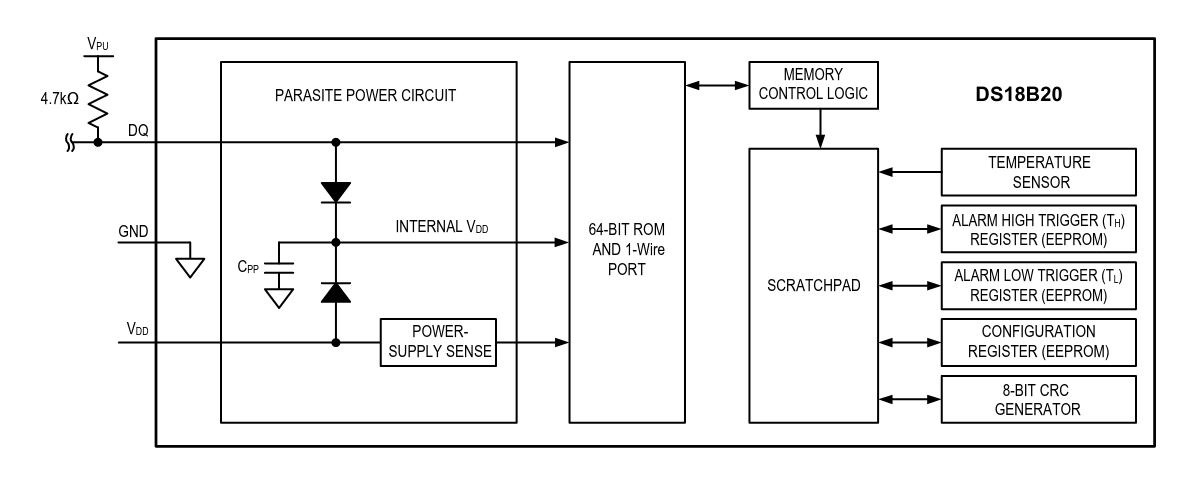
\includegraphics[width=0.8\textwidth]{/home/auan/Project/Report/Images/DS18B20_schem.png}
  \caption{Schematic of the DS18B20 sensor}
  \label{fig:sensorschem}
\end{figure}
\subsubsection{MongoDB}%
\label{ssub:mongodb}
MongoDB is an open source document database suitable for storing time-series data. This acts as the web application back-end and can also store configuration options set by the user. The database can be set up to run a daemonized process, which allows the user to get or set data whenever the server is powered on. Using the Python module PyMongo, it is possible to insert entries using JSON formatting.

\subsubsection{Systemd service}%
\label{ssub:systemd_service}
Many Linux distributions use the Systemd init daemon. While many crucial programs runs in the background by Systemd as default, it is quite straightforward to add a another service that in this case runs the Python temperature reading script. Systemd has several options to restart the service on failure, start without the need to login and redirect \verb|stdout| to the OS log called the \textit{journal}. The latter simplifies tracking how often the service behaves unexpectedly during long timespans.

\begin{lstlisting}[caption={The systemd service managing data collection}, label={systemd}]
[Unit]
# Human readable unit name
Description=Reads serially from '/dev/ttyUSB*' and puts in MongoDB

[Service]
# Command that executes script
ExecStart=/usr/bin/python /home/alarm/Project/serial_temp_to_db.py
# Redirect print() to the Linux journal
Environment=PYTHONUNBUFFERED=1
# Able to notify that the service is ready
Type=notify
Restart=always

[Install]
# Start service at boot
WantedBy=default.target
\end{lstlisting}



\subsubsection{Plotly Dash web application}%
\label{ssub:plotly_dash_web_application}
The web application consists of
\begin{enumerate}
  \item A live graph showing the $n$ most recent data points. It is updated by a timed callback function
  \item A graph showing the historical data of measurements. The user can pick start and stop times from in the span of the registered dates in the database. The data is updated if the page is refreshed.
  \item The user can set alarm levels which sends and alert email if a drastic temperature drop is detected
\end{enumerate}

Dash is an open source data visualization framework that runs in a web application. It is maintained by Plotly and build upon using their graphing software with the same name.

Each website object can be decorated with a callback function that either updates due to a time interval or through user interaction.

In order to utilize the power of Pandas, the data is loaded into a dataframe which allows many types of manipulation in areas such as statistics and signal processing.

Since the data ordered by a timestamp, it is sorted in natural order and the start and stop date can be chosen by the user.

\newpage
% How is each part of the sys interconnected?
% AVR
%   Description of drivers
%   Driver header listings
% DS18B20
%   Description of drivers
%   Driver header listings
\section{Result and discussions}%
\label{sec:result_and_discussions}

%Since the data is accessed through a datetime formatted key, it is.
The resulting product is an open-source temperature monitoring system suitable for beer fermentation. Users of the web application can filter through time-series data by filtering the start and end date using callback functions communicating with the database. In order to set an alarm level for detecting a temperature drop, these callback functions are also used to write a non-volatile setting to the database. This is helping the brewer to avoid oxidation through the airlock caused by back pressure.
Standard features provided by the Plotly library lets the user zoom and mouse-hover above the data points in order to receive immediate information about the temperature reading. 

Viewing the unfiltered data points gives an overall view of the temperature fluctuations during longer timespans. When viewing in smaller time windows, the signal is in need of filtering by the MCU to reduce noise and provide a smoother curve.



\newpage
% How did it work out? Is it a finished product?
\section{Conclusions and futher work}%
\label{sec:conclusions_and_futher_work}

The system provides a user-friendly front end where the collected temperature data of the beer can be visualized, accessed and monitored through custom settings. If the temperature drops and triggers the alarm, an email is sent containing information about the difference of the two latest temperature readings. The choice of the main two programming languages, Python and C, proved to be sufficient with a few additions of basic Linux scripting. The dependencies for the C programs was easy to track. Python, on the other hand, relies on many module dependencies which makes it hard to track. This is a trade-off when wrapping many functionalities consistently within one programming or scripting language.

\subsection{Improvements}%
\label{sub:improvements}
While there exist a multitude of possible extensions to the system, many of the existing features can be improved or optimized.

\begin{enumerate}
 \item Pre-processing the data through a filter on the MCU is more efficient compared to post-processing larger parts on the dataset while also running the web application. The post-processing was made using the \verb|savgol| filter from the Numpy Python library and could have been improved by tuning an optimal resampling size. 
 \item If the data is filtered by the RPi, the trace is toggled by the user and only computed when chosen. When filtering a large time-series, the user should be able to set the use choose a dynamic window size.
 \item Since the MCU only polls for an input every hour it could be possible to implement a rule to let the Linux kernel power the USB connecting to the MCU shortly before asking for a measurement.
 \item The server can be deployed to be accessed through the internet and lets the user remotely monitor the temperature in real time. This was not investigated due to security issues.
 \item Presenting the statistics of the data in a separate area.
\end{enumerate}

\newpage
% Optimizations? DB and data filtering alternatives.
% Power saving
% Redirection to internet

\input{Sections/appendices.tex}
% Code listings
\newpage
\printbibliography
\newpage
\mylisting[language=c]{~/Project/DS18B20_UART/src/main.c}
\mylisting[language=c]{~/Project/DS18B20_UART/src/uart.c}
\mylisting[language=c]{~/Project/DS18B20_UART/src/onewire.c}
\mylisting[language=c]{~/Project/DS18B20_UART/inc/uart.h}
\mylisting[language=c]{~/Project/DS18B20_UART/inc/onewire.h}
\mylisting[language=python]{~/Project/livedb.py}
\mylisting[language=python]{~/Project/serial_temp_to_db.py}
\end{document}
